%
% Portuguese-BR vertion
% 
\documentclass{article}

\usepackage{ipprocess}
% Use longtable if you want big tables to split over multiple pages.
\usepackage{longtable}
\usepackage[utf8]{inputenc} 
\usepackage[brazil]{babel} % Uncomment for portuguese
\usepackage{siunitx}

\sisetup{math-micro=\text{µ},text-micro=µ}


\sloppy

\graphicspath{{./pictures/}} % Pictures dir
\makeindex
\begin{document}

\DocumentTitle{Documento de Arquitetura}
\Project{Microarquitetura}
\Organization{Chip over the Hill}
\Version{Build 1.5}

\capa
\newpage
\newpage

%%%%%%%%%%%%%%%%%%%%%%%%%%%%%%%%%%%%%%%%%%%%%%%%%%
%% Revision History
%%%%%%%%%%%%%%%%%%%%%%%%%%%%%%%%%%%%%%%%%%%%%%%%%%
\chapter*{Histórico de Revisões}
\begin{center}
	\begin{longtable}[pos]{|m{2cm} | m{8cm} | m{4cm}|} 
		\hline
		\cellcolor[gray]{0.9}
		\textbf{Date} & \cellcolor[gray]{0.9}\textbf{Descrição} & \cellcolor[gray]{0.9}\textbf{Autor(s)}\\ \hline
		\endfirsthead
		\hline
		\multicolumn{3}{|l|}%
		{{\bfseries continuação da página anterior}} \\
		\hline
		\cellcolor[gray]{0.9}
		\textbf{Date} & \cellcolor[gray]{0.9}\textbf{Descrição} & \cellcolor[gray]{0.9}\textbf{Autor(s)}\\ \hline
		\endhead
		
		\multicolumn{3}{|r|}{{continua na próxima página}} \\ \hline
		\endfoot
		
		\hline
		\endlastfoot
		
      14/09/2015 &  Criação do documento & Lucas Morais \\ \hline  
      15/09/2015 & Adição das tabelas de instrução & Lucas Morais \\ \hline
      15/09/2015 & Adição das imagens & Lucas Morais \\ \hline
      15/09/2015 &  Criação das tabelas de entrada e saída dos módulos & Patricia Gomes \\ \hline
      30/09/2015 & Criação de descrição OP Jump & Fábio Almeida\\ \hline

    \end{longtable}
\end{center}

% TOC instantiation
\tableofcontents

%%%%%%%%%%%%%%%%%%%%%%%%%%%%%%%%%%%%%%%%%%%%%%%%%%
%% Document main content
%%%%%%%%%%%%%%%%%%%%%%%%%%%%%%%%%%%%%%%%%%%%%%%%%%
\newpage
\section{Introdução}
  
 Este documento descreve a arquitetura do projeto baseado no \si\micro Risc, incluindo especificações do circuitos internos. Este documento também apresenta definições de entrada e saída, conjunto de instruções e a arquitetura geral do processador. O presente documento tem como objetivo especificar a arquitetura do processador de proposito geral que será implementado em FPGA.

\subsection{Visão Geral do Documento}
O presente documento é apresentado como segue:
  \begin{itemize}
       \item \textbf{Seção 2 --} especifica a representação da visão arquitetural;
       \item \textbf{Seção 3 --} descreve os objetivos e as restrições arquiteturais;
       \item \textbf{Seção 4 --} apresenta a visão de componentes do projeto do processador;
       \item \textbf{Seção 5 --} apresenta a visão lógica do projeto do processador;
       \item \textbf{Referências --} apresenta  as  referências  utilizadas  para  a  elaboração  deste documento;
  \end{itemize}
  
  \newpage
  % inicio da tabela de acronimos e abreviacoes do documento
  \subsection{Acrônimos e Abreviações}
    \FloatBarrier
    \begin{table}[H]
      \begin{center}
        \begin{tabular}[pos]{|m{2cm} | m{12cm}|} 
          \hline
          \cellcolor[gray]{0.9}\textbf{Sigla} & \cellcolor[gray]{0.9}\textbf{Descrição} \\ \hline
             PC       &  Contador de Programa (\textit{Program Counter})\\ \hline
             ULA      &  Unidade Lógica e Aritmética\\ \hline
             UC      &  Unidade de Controle\\ \hline
             OPCODE  &  \textit{Operation Code}\\ \hline
             LW      &  \textit{Load Word}\\ \hline
             SW      &  \textit{Store Word}\\ \hline
             RISC     & \textit{Reduced Instruction Set Computer}\\ \hline
             GPR    &   \textit{General Purpose Register}\\ \hline
             FPGA   & \textit{Field Gate Programmable Array}\\ \hline
             GPPU   & \textit{General Purpose Processing Unit}\\ \hline
             HDL    & \textit{Hardware Description Language}\\ \hline
             ISA    & \textit{Instruction Set Architecture}\\ \hline
             IF     & \textit{Instruction Fetch}\\ \hline
             ID     & \textit{Instruction Deconding}\\ \hline
             EX     & \textit{Execute}\\ \hline
             WB     & \textit{Write Back}\\ \hline
             Const  & \textit{Constante}\\ \hline
             Const8 & \textit{Constante de 8 bits}\\ \hline
             TF & \textit{Testador de Flag}\\ \hline
        \end{tabular}
      \end{center}
    \end{table}  
  % fim
  
  
  \newpage
\section{Visão Geral da Arquitetura}


\subsection{Datapath}
Nesta seção é mostrada o Datapath completo do nosso processador baseado em \si\micro Risc. 

  Trocar o datapath aqui
\begin{figure}[H]
	\centering
	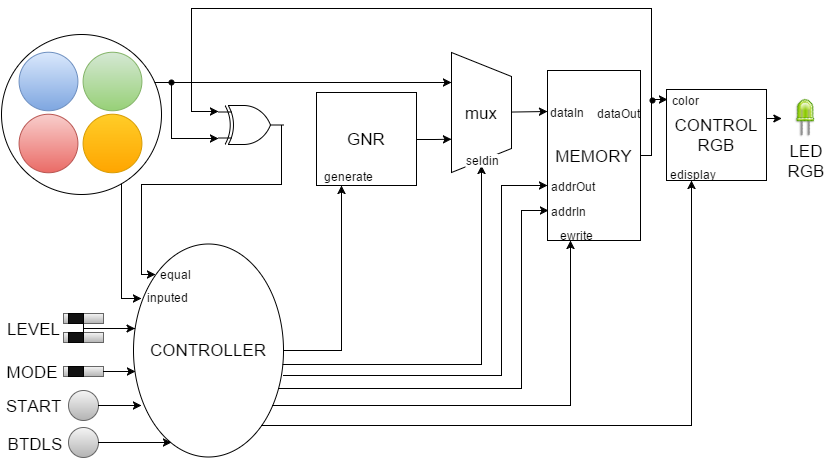
\includegraphics[width=\textwidth]{./pictures/datapath.png}
\end{figure}


\section{Instruções}
\subsection{Instruções lógico e aritméticas}
    Descrever aqui o funcionamento geral das instruções 

\subsection{Instruções com constantes}
   Descrever aqui o funcionamento geral das instruções com constante

\subsection{Instruções de acesso à memória}
    Descrever aqui o funcionamento dessas instruções

\subsection{Instruções de jump}
    Descrever aqui todos os jumps
    
%\begin{itemize}
    Detalhamento das instruções, assim como o layout da instrução, estão mostrados no documento de Especificação.
    \newpage
	\begin{table}[H]
	\centering
	\begin{tabular}{|c|m{6cm}|c|c|}
  	\hline 
  	\textbf{CÓDIGO} & \textbf{OPERAÇÃO} & \textbf{MNEMÔNICO} & \textbf{FLAGS ATUALIZADAS} \\ 
  	\hline   	
  	00000 & C = A + B & add c, a, b & todas \\ \hline
  	00001 & C = A + B + 1 & addinc, c, a, b & todas \\ \hline
  	00011 & C = A + 1 & inca c, a & todas \\ \hline
  	00100 & C = A - B - 1 & subdec c, a, b & todas \\ \hline
  	00101 & C = A - B & sub c, a, b & todas \\ \hline
  	00110  & C = A - 1 & deca c, a & todas \\ \hline
  	01000 & C = Deslocamento Lógico Esq. (A) & lsl c, a & S, C, Z \\ \hline
  	01001 & C = Deslocamento Aritmético Dir. (A) & asr c, a & S, C, Z \\ \hline
  	10000 & C = 0 & zeros c & Z \\ \hline
    10001 & C = A\&B & and c, a, b & Z, S \\ \hline
    10010 & C = !A\&B & andnota c, a, b & Z, S \\ \hline
    10011 & C = B & passb c, b & nenhuma \\ \hline
    10100 & C = A\&!B & andnotb c, a, b & Z, S \\ \hline
    10101 & C = A & passa c, a & Z, S \\ \hline
    10110 & C = A xor B & xor c, a, b & Z, S \\ \hline
    10111 & C = A |B & or c, a, b & Z, S \\ \hline
    11000 & C = !A\&!B & nand c, a, b & Z, S \\ \hline
    11001 & C = !(A xor B) & xnor c, a, b & Z, S \\ \hline
    11010 & C = !A & passnota c, a & Z, S \\ \hline
    11011 & C = !A|B & ornota c, a, b & Z, S \\ \hline
    11100 & C = !B & passnotb c, b & Z, S \\ \hline
    11101 & C = A|!B & ornotb c, a, b & Z, S \\ \hline
    11110 & C = !A|!B & nor c, a, b & Z, S \\ \hline
    11111 & C = 1 & ones c & nenhuma \\ \hline
  	\end{tabular} 
  	\caption{Instruções lógico e aritméticas}
  \end{table}
  \newpage    


\subsection{Operações com constantes}
\begin{table}[H]
	\centering
	\begin{tabular}{|c|m{6cm}|c|c|}
  	\hline 
  	\textbf{Formato} & \textbf{Operação} & \textbf{Mnemônico} \\ 
  	\hline 
  	I & C = Constante & loadlit c, Const \\ \hline
  	II & C = Const8 | (C\&0x00) & lcl c, Const8 \\ \hline
  	II & C = (Const8 « 8) | (C\&0x00 ) & lch c, Const8 \\ \hline
  	\end{tabular} 
  	\caption{Operações com constantes}
  \end{table}
  
Detalhamento das instruções, assim como o layout da instrução, estão mostrados no documento de Especificação.

\subsection{Operações de Acesso à Memória}
\begin{table}[H]
	\centering
	\begin{tabular}{|c|m{6cm}|c|c|}
  	\hline 
  	\textbf{OP} & \textbf{Operação} & \textbf{Mnemônico} \\ 
  	\hline 
  	01010 & C = Mem[A] & load c, a \\ \hline
  	01011 & Mem[A] = B & store a, b \\ \hline
  	\end{tabular} 
  	\caption{Operações de Acesso à Memória}
  \end{table}
  
  Detalhamento das instruções, assim como o layout da instrução, estão mostrados no documento de Especificação.
  A instrução de Load segue o seguinte datapath:
  \begin{figure}[H]
	\centering
	\includegraphics[scale=0.58]{./pictures/load.png}
\end{figure}  
\newpage
A instrução de Store segue o seguinte datapath:
\begin{figure}[H]
	\centering
	\includegraphics[scale=0.58]{./pictures/store.png}
\end{figure}  
  
  
  \newpage
  
  
  
\section{Uidades Internas}
 \subsection{Contador de Programa (PC)}
    O Contador de Programa (PC) é o registrador de 16 bits que armazena o endereço da próxima instrução a ser executada.
 \FloatBarrier
    \begin{table}[H]
      \begin{center}
        \begin{tabular}[pos]{|m{7cm} | m{7cm}|} 
          \hline
          \cellcolor[gray]{0.9}\textbf{Entradas} & \cellcolor[gray]{0.9}\textbf{Saídas} \\ \hline
            Resultado do somador & Endereço na memória de instrução\\ \hline
            Sinal controlePC & \\ \hline
        \end{tabular}
      \end{center}
    \end{table}  
    
 \subsection{Memória de Instruções}
    Tem uma capacidade de endereçamento de 16 bits. Sendo que esta pode armazenar até 65536 instruções de programa para execução no Processador de propósito geral. Tem como funcionalidade armazenar o programa a ser executado (as sequência de instruções a ser executada).
  \FloatBarrier
    \begin{table}[H]
      \begin{center}
        \begin{tabular}[pos]{|m{7cm} | m{7cm}|} 
          \hline
          \cellcolor[gray]{0.9}\textbf{Entradas} & \cellcolor[gray]{0.9}\textbf{Saídas} \\ \hline
            Endereço & A instrução \\ \hline
        \end{tabular}
      \end{center}
    \end{table}  
    
 \subsection{Banco de Registradores}
    O banco de registradores consiste de oito registradores de propósito geral.
  \FloatBarrier
    \begin{table}[H]
      \begin{center}
        \begin{tabular}[pos]{|m{7cm} | m{7cm}|} 
          \hline
          \cellcolor[gray]{0.9}\textbf{Entradas} & \cellcolor[gray]{0.9}\textbf{Saídas} \\ \hline
            Endereço dos registradores & Os operandos\\ \hline
            Dado a ser escrito no registrador de escrita & \\ \hline
            Sinal BrSelESa & \\ \hline
            Sinal BrSelSb & \\ \hline
            Sinal BrHabEscrita & \\ \hline
        \end{tabular}
      \end{center}
    \end{table}  
    
 \subsection{Extensor de sinal}
    O extensor de sinal é utilizado na operações com constantes e também no Jump. 
  \FloatBarrier
    \begin{table}[H]
      \begin{center}
        \begin{tabular}[pos]{|m{7cm} | m{7cm}|} 
          \hline
          \cellcolor[gray]{0.9}\textbf{Entradas} & \cellcolor[gray]{0.9}\textbf{Saídas} \\ \hline
            Uma palavra de 11 bits & Uma palavra de 16 bits \\ \hline
            Uma palavra de 8 bits & \\ \hline
            Sinal Excontrole & \\ \hline
        \end{tabular}
      \end{center}
    \end{table}  
    
 \subsection{Multiplexador 1}
  \FloatBarrier
    \begin{table}[H]
      \begin{center}
        \begin{tabular}[pos]{|m{7cm} | m{7cm}|} 
          \hline
          \cellcolor[gray]{0.9}\textbf{Entradas} & \cellcolor[gray]{0.9}\textbf{Saídas} \\ \hline
            Sinal ControleMuxUla & Valor que sai do extensor ou a saída do operando B\\ \hline
            Valor que sai do extensor & \\ \hline
            Saída do operando B & \\ \hline
        \end{tabular}
      \end{center}
    \end{table}  
    
 \subsection{Unidade Lógica Aritmética (ULA)}
    A Unidade Lógica e Aritmética (ULA) é um circuito combinatório responsável por realizar operações aritméticas e lógicas dentro de um processador. As operações a serem executadas são determinadas por meio dos sinais de controle das suas entradas de operação, logo após os dados de entrada são computados e o resultado é obtido na saída do circuito.
  \FloatBarrier
    \begin{table}[H]
      \begin{center}
        \begin{tabular}[pos]{|m{7cm} | m{7cm}|} 
          \hline
          \cellcolor[gray]{0.9}\textbf{Entradas} & \cellcolor[gray]{0.9}\textbf{Saídas} \\ \hline
            Operando A & Resultado da operação\\ \hline
            Saída do multiplexador 1 & Flag\\ \hline
            Sinal ULAOp & \\ \hline
        \end{tabular}
      \end{center}
    \end{table}  
    
  \subsection{Memória de Dados}
    A Memória de dados é endereçada com 16 bits. Tem como propósito salvar/ler dados proveniente da instruções de acesso à memória.
  \FloatBarrier
    \begin{table}[H]
      \begin{center}
        \begin{tabular}[pos]{|m{7cm} | m{7cm}|} 
          \hline
          \cellcolor[gray]{0.9}\textbf{Entradas} & \cellcolor[gray]{0.9}\textbf{Saídas} \\ \hline
            Saída do registrador A & Informação de 16 bits\\ \hline
            Saída do registrador B & \\ \hline
            Sinal HabEscritaMem & \\ \hline
            Sinal Reset & \\ \hline
        \end{tabular}
      \end{center}
    \end{table}  
    
 \subsection{Registrador de Flags}
  \FloatBarrier
    \begin{table}[H]
      \begin{center}
        \begin{tabular}[pos]{|m{7cm} | m{7cm}|} 
          \hline
          \cellcolor[gray]{0.9}\textbf{Entradas} & \cellcolor[gray]{0.9}\textbf{Saídas} \\ \hline
            Saída de Flags da ULA & \\ \hline
            Sinal RegFlagControle & \\ \hline
        \end{tabular}
      \end{center}
    \end{table}  
    
 \subsection{Multiplexador2}
  \FloatBarrier
    \begin{table}[H]
      \begin{center}
        \begin{tabular}[pos]{|m{7cm} | m{7cm}|} 
          \hline
          \cellcolor[gray]{0.9}\textbf{Entradas} & \cellcolor[gray]{0.9}\textbf{Saídas} \\ \hline
            Saída de ULA & Valor da saída da ULA ou valor da saída da memória de dados\\ \hline
            Saída da memória de Dados & \\ \hline
            Sinal ControleMux2 & \\ \hline
        \end{tabular}
      \end{center}
    \end{table}  
    \newpage
    \subsection{Unidade de Controle (UC)}
    Esta unidade é responsável por gerar todos os sinais de controle do processador, como  sinais  de  leitura,  escrita  de  memoria  e  de  registradores  de  armazenamento temporário  interno  e  sinais  de  liberação  de  barramentos  para  endereço  e  dados  e unidades  funcionais.  As  unidades  funcionais  internas  do  processador  são  controladas por esta unidade de temporização e controle. Estes sinais de controle são enviados para as unidades funcionais após a decodificação de uma instrução.
  \FloatBarrier
    \begin{table}[H]
      \begin{center}
        \begin{tabular}[pos]{|m{4cm} | m{4cm}| m{5cm}|} 
          \hline
          \cellcolor[gray]{0.9}\textbf{Entradas} & \cellcolor[gray]{0.9}\textbf{Saídas} & 
          \cellcolor[gray]{0.9}\textbf{descrição dos sinais}\\ \hline
            Código da operação & Sinal ControlePC & Indica quando o PC apontará para a instrução seguinte \\ \hline
            Formato da operação & Sinal BrSelESa & Indica qual será a saída de A no banco de registradores ou onde será escrito o novo registro conforme o estado do sinal BrHabEscrita\\ \hline
            & Sinal BrSelSb & Indica qual será a saída de B no banco de registradores \\ \hline
            & Sinal ExControle & Indica qual será o tipo de extensão que ocorrerá no extensor de sinais\\ \hline
            & Sinal ControleMuxULA & Indica se o operando B da ULA será a saída B do banco de registradores ou a saída do extensor de sinal \\ \hline
            & Sinal ULAOp & Indica a operação que será realizada pela ULA\\ \hline
            & Sinal RegFlagControle & Indica quais as flags atualizadas pela instrução executada\\ \hline
            & Sinal BrHabEscrita & Habilita a escrita no banco de registradores \\ \hline
            & Sinal HabEscritaMem & Habilita a escrita na memória de dados\\ \hline
            & Sinal Reset & Limpa a memória de dados \\ \hline
            & Sinal ControleMux2 & Indica se o valor a ser inscrito no banco de regitradores é a saída da ULA ou a saída da memória de dados  \\ \hline
        \end{tabular}
      \end{center}
    \end{table}  
    

% Optional bibliography section
% To use bibliograpy, first provide the ipprocess.bib file on the root folder.
% \bibliographystyle{ieeetr}
% \bibliography{ipprocess}

\end{document}
